%%%%%%%%%%%%%%%%%%%%% chapter.tex %%%%%%%%%%%%%%%%%%%%%%%%%%%%%%%%%
%
% sample chapter
%
% Use this file as a template for your own input.
%
%%%%%%%%%%%%%%%%%%%%%%%% Springer-Verlag %%%%%%%%%%%%%%%%%%%%%%%%%%
%\motto{Use the template \emph{chapter.tex} to style the various elements of your chapter content.}
\chapter{Linear Regression}
\label{intro} % Always give a unique label
% use \chaptermark{}
% to alter or adjust the chapter heading in the running head

\abstract*{
    This chapter introduces the principles of linear regression as a foundation for understanding the connection between differential geometry and machine learning. A simple linear model $M(x) = W \cdot x + b$ is constructed, and a loss function is used to quantify prediction errors. The chapter details the derivation of gradients for the loss with respect to the model parameters $W$ and $b$, providing insights into how these gradients guide the optimization process.
}

\abstract{
    This chapter introduces the principles of linear regression as a foundation for understanding the connection between differential geometry and machine learning. A simple linear model $M(x) = W \cdot x + b$ is constructed, and a loss function is used to quantify prediction errors. The chapter details the derivation of gradients for the loss with respect to the model parameters $W$ and $b$, providing insights into how these gradients guide the optimization process.
}

\section{Linear Models}
\label{sec:1}
Linear regressions are a fundamental tool in statistics and machine learning for modeling the relationship between a dependent variable $y$ and one or more independent variables $x$. The simplest form of linear regression is a univariate linear model, which assumes a linear relationship between $y$ and $x$ of the form $y = W \cdot x + b$, where $W,b\in\mathbb{R}$ are real numbers. The model parameters $W$ and $b$ are learned from a dataset of input-output pairs $\{(x_i, y_i)\}_{i=1}^N$ by minimizing a loss function that quantifies the prediction errors of the model. 

A more general form of the linear model is:
$$M(x) = W \cdot x + b,$$
where:
\begin{itemize}
    \item $W$ is a \textbf{weight matrix} of shape $m \times d$,
    \item $x$ is a $d$-dimensional input vector,
    \item $b$ is an $m$-dimensional \textbf{bias vector}.
\end{itemize}

Here, the model $M(x)$ outputs an $m$-dimensional vector prediction. This flexibility allows linear regression to handle scenarios where the model predicts multiple outputs simultaneously, making it applicable to a wide range of machine learning tasks. We begin by studying the univariate case.

\section{Univariate Linear Models}
\label{sec:2}
% Always give a unique label
% and use \ref{<label>} for cross-references
% and \cite{<label>} for bibliographic references
% use \sectionmark{}
% to alter or adjust the section heading in the running head
Let's construct some data to work with that follows a somewhat linear trend and build a machine-learning model from scratch. We'll take the function $f(x)=x^2+2\cdot x+1$ over a random sample of points in $[0,10]$ and add some uniform noise.

% \begin{lstlisting}[language=Python, caption=Python example]
%  def f(x):
%     return x**2 + 2*x + 1
% \end{lstlisting}

\begin{codeblock}
def f(x):
    return x**2 + 2*x + 1

# Plot using matplotlib
import matplotlib.pyplot as plt
import numpy as np
import random

# Define the true function
def f(x):
    return x**2 + 2*x + 1

# Generate data
np.random.seed(42)
x = np.linspace(0, 10, 200)
y_true = f(x)
y_data = y_true + np.random.uniform(-10, 10, size=x.shape)

# Plot from 0 to 10
plt.xlim(0, 10)
plt.plot(x, y_data, 'o')
plt.plot(x, y_true)
plt.show()
\end{codeblock}

\begin{figure}[H]
\centering
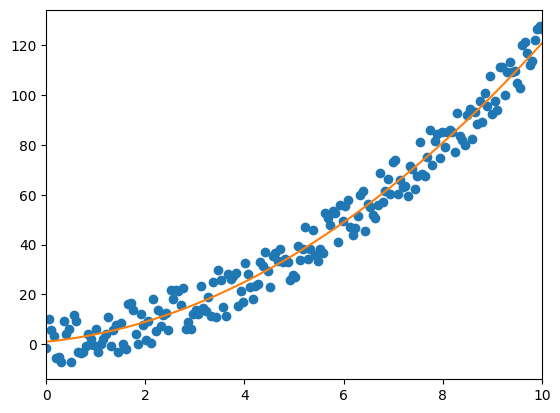
\includegraphics[width=200pt]{Regression/img/output_2_0.png}
\caption{Data generated from the function $f(x)=x^2+2\cdot x+1$ with added noise.}
\label{fig:linear1}
\end{figure}

In Figure \ref{fig:linear1}, the \textit{best fit} for this data is the function we used to construct it. Of course, we usually don't know the equation for the best fit beforehand, but our goal is to create a model to approximate this line as closely as possible. 

Let us start by constructing a simple machine-learning model for linear regression with no hidden layers, which essentially means there are no intermediate computations between the input and the output in our model.

Our goal is to build a machine-learning model 
$M:[0,10]\to\mathbb{R}$ of the form $$M(x) = W\cdot x + b,$$ where $W\in\mathbb{R}$ and $b\in\mathbb{R}$. Here, $W$ is called the **weight** and $b$ is called the **bias**.   

Here, we define our linear model:

\begin{codeblock}
# Linear model
def linear_model(x, w, b):
    return w * x + b
\end{codeblock}

In machine-learning, a model is initialized with random weights and biases, which are then corrected during training by minimizing a **loss function**. Let's start by choosing some random $W$ and $b$.

\begin{codeblock}
# Initialize parameters
w = random.uniform(-1, 1)  # Random initial weight
b = random.uniform(-1, 1)  # Random initial bias


print(f'Initial weight: {w}')
print(f'Initial bias: {b}')
\end{codeblock}
\texttt{Initial weight: 0.918163880835746\\
Initial bias: 0.6882870252000235}

Given that the weight and bias was chosen at random, we don't expect it to perform very well on our data, and indeed that is the case, as shown in the image below.

\begin{figure}[H]
\centering
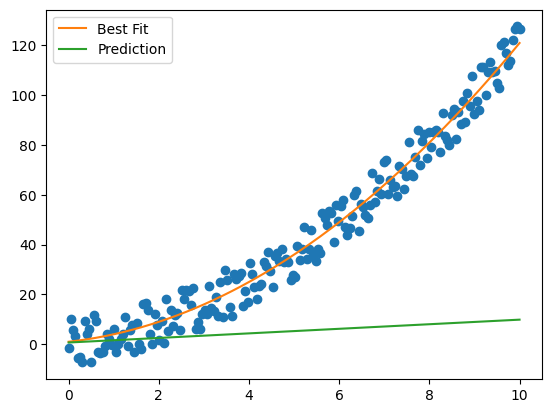
\includegraphics[width=200pt]{Regression/img/output_6_0.png}
\caption{Initial model prediction with random weight and bias.}
\label{fig:linear2}
\end{figure}

Let's work on improving the model. Improving our model will involve tweaking $W$ and $b$ to better fit the model using a process called \textbf{gradient descent}.

\subsection{Gradient Descent for Univariate Linear Models}
\label{subsec:2}
We first define a \textbf{loss function} to measure how our model is performing. This function will quantify the difference between the model's predictions and the actual data. A common loss function for linear regression is the \textit{Mean Squared Error} (MSE), which is defined as:
$$\mathcal{L} = MSE = \frac{1}{N}\sum_{i=1}^N\left(y_\text{i,pred} - y_\text{i,true}\right)^2.$$

\begin{codeblock}

# Mean Squared Error Loss
def mse_loss(y_pred, y_true):
    return np.mean((y_pred - y_true)**2)

print(f'50th sample target: {y_data[50]}')
print(f'50th prediction: {y_pred[50]}')
print(f'Loss at 50th sample: {mse_loss(y_pred[50], y_data[50])}')

print('Total Loss over all samples:', mse_loss(np.array(y_pred), np.array(y_data)))
\end{codeblock}
\texttt{50th sample target: 21.729790078081002 \\
50th prediction: 2.995231449410441 \\
Loss at 50th sample: 350.9836870110946 \\
Total Loss over all samples: 2660.1490298370586 \\
}

Our goal is to minimize this loss function. 

One thing to note about this loss function is that it is a differentiable function. Recal from vector calculus that the \textbf{gradient} of a differentiable funtion $f$ is a vector field $\nabla f$ whose value at point $p$ is a vector that points towards the direction of steepest ascent. 

Understanding the gradients of the loss function with respect to the model parameters—specifically, the weight $W$ and bias $b$—is crucial in machine learning, particularly when employing optimization techniques like gradient descent. Our goal is to minimize the loss function. 

The gradients $\frac{\partial \mathcal{L}}{\partial W}$ and $\frac{\partial \mathcal{L}}{\partial b}$ indicate how sensitive the loss function $\mathcal{L}$ is to changes in the parameters $W$ and $b$. In essence, they provide the direction and rate at which $\mathcal{L}$ increases or decreases as we adjust these parameters.

By computing these gradients, we can iteratively update $W$ and $b$ to minimize the loss function, thereby improving the model's performance. This process is the foundation of the gradient descent optimization algorithm.

\subsubsection{Gradients}
\begin{enumerate}
    \item \textit{Gradient with Respect to Weight $W$:}

    The partial derivative $\frac{\partial \mathcal{L}}{\partial W}$ measures how the loss changes concerning the weight $W$. A positive derivative suggests that increasing $W$ will increase the loss, while a negative derivative indicates that increasing $W$ will decrease the loss. By moving $W$ in the direction opposite to the gradient, we can reduce the loss.

    If $x_i$ is the i-th data point, let $y_{i,\text{pred}} = W \cdot x_i + b$ be the predicted value for the $i$-th data point while $y_{i,\text{true}}$ denotes the true value. Mathematically, this gradient is computed as:
    \begin{align*}
        \frac{\partial \mathcal{L}}{\partial W} &= \frac{\partial}{\partial W}\left( \frac{1}{N}\sum_{i=1}^N(y_{i,\text{pred}} - y_{i,\text{true}})^2\right) \nonumber \\
        & = \frac{1}{N}\sum_{i=1}^N\frac{\partial}{\partial W}(y_{i,\text{pred}} - y_{i,\text{true}})^2 \qquad \text{(Additive property of derivatives)} \nonumber \\
        & = \frac{1}{N}\sum_{i=1}^N\frac{\partial}{\partial W}((W\cdot x_i + b) - y_{i,\text{true}})^2 \nonumber \\
        & = \frac{1}{N}\sum_{i=1}^N 2\cdot((W\cdot x_i + b) - y_{i,\text{true}})\cdot (x_i) \qquad \text{(Chain rule)} \nonumber \\
        & = \frac{2}{N}\sum_{i=1}^N(y_{i,\text{pred}} - y_{i,\text{true}})\cdot x_i.
    \end{align*}

    Thus, we find that 
    \begin{equation}
        \frac{\partial \mathcal{L}}{\partial W} = \frac{2}{N}\sum_{i=1}^N(y_{i,\text{pred}} - y_{i,\text{true}})\cdot x_i.
        \label{eq:gradient_w}
    \end{equation}
    
    \item \textit{Gradient with Respect to Bias $ b $:}

    Similarly, the partial derivative $\frac{\partial \mathcal{L}}{\partial b}$ measures how the loss changes concerning the bias $b$. Adjusting $b$ in the direction opposite to this gradient will also help in minimizing the loss.

    This gradient is computed as:
    \begin{equation}
        \frac{\partial \mathcal{L}}{\partial b} = \frac{2}{N}\sum_{i=1}^N(y_{i,\text{pred}} - y_{i,\text{true}}).
        \label{eq:gradient_b}
    \end{equation}

    Proof of this equation is left as an exercise to the reader.
\end{enumerate}
\pagebreak
With that, we can compute the gradients in Python:

\begin{codeblock}
# Compute gradients
def compute_gradients(x, y_true, w, b):
    y_pred = linear_model(x, w, b)
    error = y_pred - y_true
    dw = 2 * np.mean(error * x)
    db = 2 * np.mean(error)
    return dw, db
\end{codeblock}

Now that we have a way of computing the partial derivatives of $\mathcal{L}$ with respect to $W$ and $b$, we can visualize the \textit{gradient field}. For a given $p=(W, b) \in \mathbb{R}^2$, the gradient $\nabla \mathcal{L}$ at $p$ is a vector that points towards the rate of fastest increase. In the following code, we compute these vectors on a grid. We also include a 2D contour plot of the loss function $\mathcal{L}$. Our initial weight $W$ and bias $b$ are marked on the plot by a red dot.

\begin{codeblock}
import numpy as np
import matplotlib.pyplot as plt

# Gradient Descent parameters
alpha = 0.001  # Learning rate
epochs = 1000  # Number of iterations

# Create a grid of w and b values for contour and quiver plotting
w_vals = np.linspace(-10, 20, 100)
b_vals = np.linspace(-20, 10, 100)
W, B = np.meshgrid(w_vals, b_vals)

# Compute the loss for each combination of w and b in the grid
Z = np.array([mse_loss(linear_model(x, w, b), y_data) for w, b in zip(np.ravel(W), np.ravel(B))])
Z = Z.reshape(W.shape)

# Compute the gradient field
dW = np.zeros(W.shape)
dB = np.zeros(B.shape)
for i in range(W.shape[0]):
    for j in range(W.shape[1]):
        dw, db = compute_gradients(x, y_data, W[i, j], B[i, j])
        dW[i, j] = dw
        dB[i, j] = db

# Plot the cost function contour, gradient field, and gradient descent path
plt.figure(figsize=(12, 8))

# Contour plot of the loss function
cp = plt.contour(W, B, Z, levels=np.logspace(-1, 3, 20), cmap='viridis')
plt.colorbar(cp)
plt.xlabel('Weight (w)')
plt.ylabel('Bias (b)')
plt.title('Cost Function Contour, Gradient Field, and Gradient Descent Path')

# Quiver plot of the gradient field
plt.quiver(W, B, dW, dB, angles='xy', scale_units='xy', scale=1, color='blue', alpha=0.5)
# plot initial weight, bias
plt.plot(w, b, 'ro', label='Initial (weight, bias)')
plt.legend()
plt.grid(True)
plt.show()
\end{codeblock}

\begin{figure}
\centering
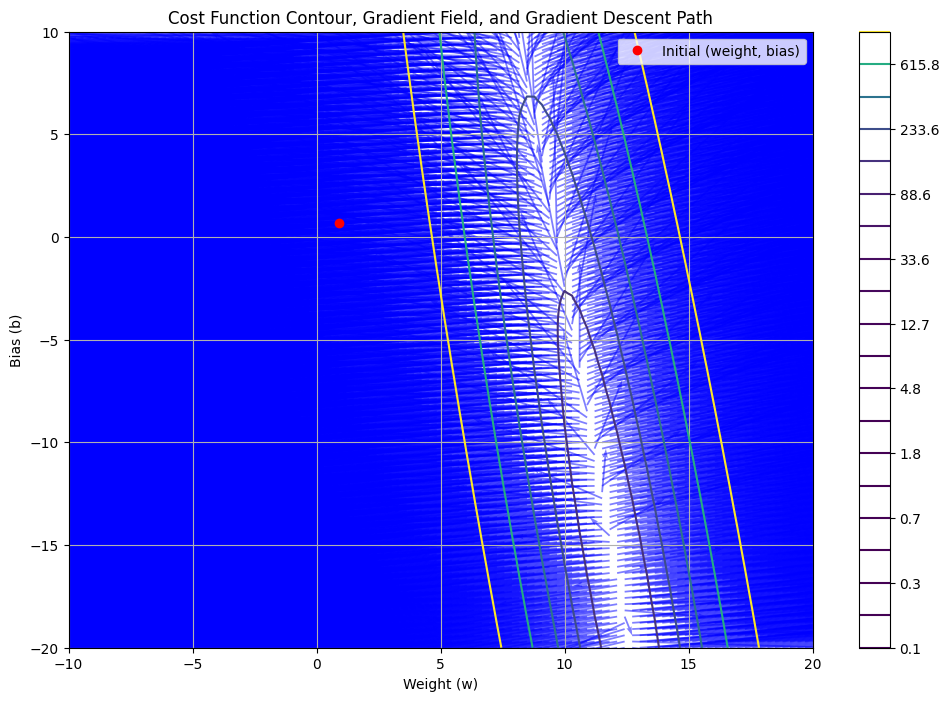
\includegraphics[width=300pt]{Regression/img/output_12_0.png}
\caption{Contour plot of the loss function, gradient field, and gradient descent path.}
\label{fig:linear3}
\end{figure}

Since our goal is to minimize the loss function and these vectors are pointing towards the steepest ascent of the loss function with respect to $W$ and $b$, we minimize by moving in the opposite direction of the gradients. This process is fundamental to optimization algorithms like gradient descent and is refered to as \textbf{backward propogation} within machine-learning.

\subsubsection{Gradient Descent \& Backward Propagation}
\label{subsubsec:2}
\textbf{Gradient descent} is an optimization algorithm that iteratively updates the model parameters in the direction opposite to the gradients of the loss function. This process continues until the loss is minimized. \textbf{Backward propagation} is the process of computing these gradients and updating the model parameters.

The parameter updates are performed iteratively using the following rules:
\begin{enumerate}
    \item  Weight update:
    $$W \leftarrow W - \alpha \frac{\partial \mathcal{L}}{\partial W}$$
   Here, $\alpha$ is the learning rate, a hyperparameter that controls the step size of each update. The term $\frac{\partial \mathcal{L}}{\partial W}$ represents the gradient of the loss function with respect to the weight. By subtracting this scaled gradient from the current weight, we move $ W $ in the direction that decreases the loss.

    \item Bias update:
    $$b \leftarrow b - \alpha \frac{\partial \mathcal{L}}{\partial b}$$
    Similarly, $\frac{\partial \mathcal{L}}{\partial b}$ is the gradient of the loss function with respect to the bias. Updating $b$ in this manner adjusts the model's predictions to better fit the data.
\end{enumerate}

The \textbf{learning rate} determines how large a step we take in the direction of the negative gradient. A small $\alpha$ leads to slow convergence, while a large $\alpha$ might cause overshooting the minimum, leading to divergence. Choosing an appropriate learning rate is crucial for effective training.

The gradients $\frac{\partial \mathcal{L}}{\partial W}$ and $\frac{\partial \mathcal{L}}{\partial b}$ indicate the direction in which the loss function increases most rapidly. By moving in the opposite direction (hence the subtraction), we aim to find the parameters that minimize the loss.

We repeat this process over and over again. Each time we do it is referred to as an \textbf{epoch}. 

\begin{codeblock}
import numpy as np
import matplotlib.pyplot as plt

# Assuming x and y_data are your input features and target values respectively

# Define the linear model
def linear_model(x, w, b):
    return w * x + b

# Define the loss function (Mean Squared Error)
def mse_loss(y_pred, y_true):
    return np.mean((y_pred - y_true) ** 2)

# Compute gradients
def compute_gradients(x, y_true, w, b):
    y_pred = linear_model(x, w, b)
    error = y_pred - y_true
    dw = 2 * np.mean(error * x)
    db = 2 * np.mean(error)
    return dw, db

# Gradient Descent parameters
alpha = 0.001  # Learning rate
epochs = 2000  # Number of iterations

# Store parameters for plotting
w_history = [w]
b_history = [b]
loss_history = [mse_loss(linear_model(x, w, b), y_data)]

# Gradient Descent loop
for epoch in range(epochs):
    dw, db = compute_gradients(x, y_data, w, b) 
    w = w - alpha * dw # Update the weight
    b = b - alpha * db # Update the bias

    w_history.append(w) # Add to weight tracker
    b_history.append(b) # Add to bias tracker
    loss_history.append(mse_loss(linear_model(x, w, b), y_data)) # Add overall loss to loss tracker

# Convert history lists to numpy arrays for easier slicing
w_history = np.array(w_history)
b_history = np.array(b_history)

# Create a grid of w and b values for contour and quiver plotting
w_vals = np.linspace(-10, 20, 100)
b_vals = np.linspace(-20, 10, 100)
W, B = np.meshgrid(w_vals, b_vals)

# Compute the loss for each combination of w and b in the grid
Z = np.array([mse_loss(linear_model(x, w, b), y_data) for w, b in zip(np.ravel(W), np.ravel(B))])
Z = Z.reshape(W.shape)

# Compute the gradient field
dW = np.zeros(W.shape)
dB = np.zeros(B.shape)
for i in range(W.shape[0]):
    for j in range(W.shape[1]):
        dw, db = compute_gradients(x, y_data, W[i, j], B[i, j])
        dW[i, j] = dw
        dB[i, j] = db

# Print initial (weight, bias)
print(f'Initial (weight, bias): ({w_history[0]}, {b_history[0]})')
# Print final (weight, bias)
print(f'Final (weight, bias): ({w_history[-1]}, {b_history[-1]})')

# Plot the cost function contour, gradient field, and gradient descent path
plt.figure(figsize=(12, 8))

# Contour plot of the loss function
cp = plt.contour(W, B, Z, levels=np.logspace(-1, 3, 20), cmap='viridis')
plt.colorbar(cp)
plt.xlabel('Weight (w)')
plt.ylabel('Bias (b)')
plt.title('Cost Function Contour, Gradient Field, and Gradient Descent Path')

# Quiver plot of the gradient field
plt.quiver(W, B, dW, dB, angles='xy', scale_units='xy', scale=1, color='blue', alpha=0.5)

# Plot the gradient descent path
plt.plot(w_history, b_history, 'ro-', markersize=3, linewidth=1, label='Gradient Descent Path')
# Plot the initial weight, bias
plt.plot(w_history[0], b_history[0], 'ro', label='Initial (weight, bias)')

# Add arrows to indicate direction of descent
for i in range(1, len(w_history)):
    plt.arrow(w_history[i-1], b_history[i-1],
                w_history[i] - w_history[i-1],
                b_history[i] - b_history[i-1],
                head_width=0.05, head_length=0.1, fc='red', ec='red')

plt.legend()
plt.grid(True)
plt.show()
\end{codeblock}

\texttt{\small{Initial (weight, bias): (0.918163880835746, 0.6882870252000235)\\
Final (weight, bias): (11.090173700216313, -9.650829435811533)
}}

\begin{figure}[H]
\centering
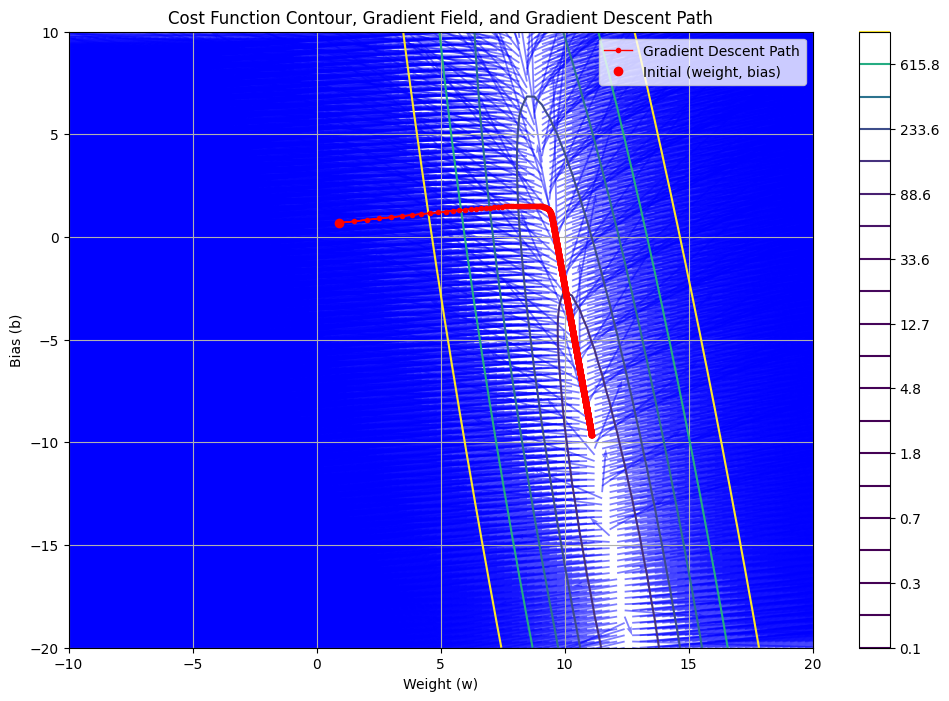
\includegraphics[width=300pt]{Regression/img/output_15_1.png}
\caption{Contour plot of the loss function, gradient field, and gradient descent path.}
\label{fig:linear4}
\end{figure}

Since our weight $W$ and bias $b$ together form a point $(W,b)\in\mathbb{R}^2$, the loss function $\mathcal{L}$ forms a 3-dimensional surface. The visualization below shows the path taken during gradient descent on the surface of the loss function $\mathcal{L}$. The initial point $(W,b)$ is in green. The path moves towards $\mathcal{L}$'s minimum.

\begin{figure}[H]
\centering
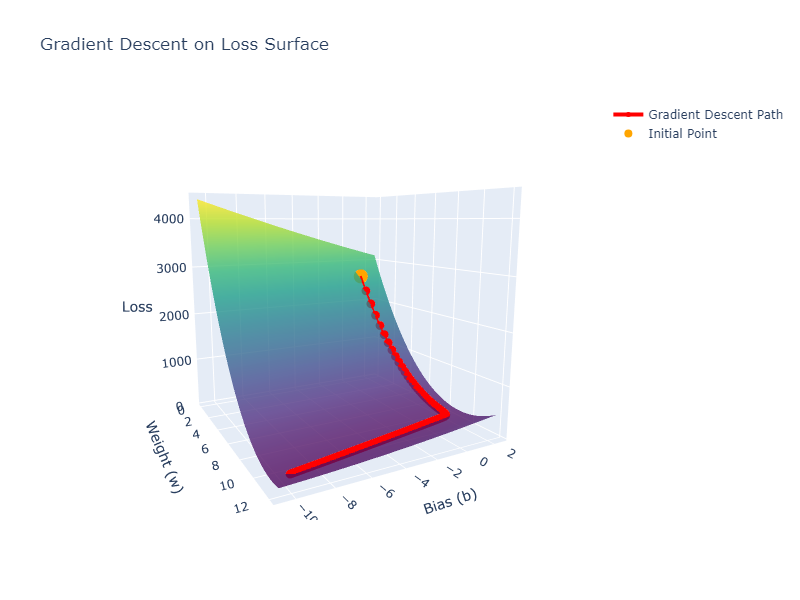
\includegraphics[width=400pt]{Regression/img/gradient-surface-plot-1.png}
\caption{Gradient descent path on the loss function surface.}
\label{fig:linear5}
\end{figure}

Finally, we visualize our initial (green) and final (red) linear model on a graph, alongside the data and true line of best fit (orange).

\begin{figure}[H]
\centering
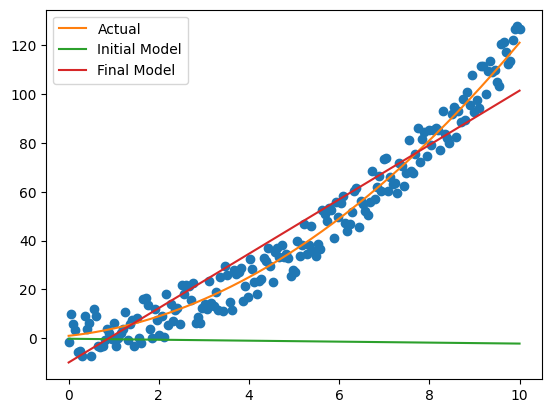
\includegraphics[width=300pt]{Regression/img/output_19_0.png}
\caption{Initial and final linear models compared to the true line of best fit.}
\label{fig:linear6}
\end{figure}

%%%%%%%%%%%%%%%%%%%%%%%%% referenc.tex %%%%%%%%%%%%%%%%%%%%%%%%%%%%%%
% sample references
% %
% Use this file as a template for your own input.
%
%%%%%%%%%%%%%%%%%%%%%%%% Springer-Verlag %%%%%%%%%%%%%%%%%%%%%%%%%%
%
% BibTeX users please use
% \bibliographystyle{}
% \bibliography{}
%
\biblstarthook{In view of the parallel print and (chapter-wise) online publication of your book at \url{www.springerlink.com} it has been decided that -- as a genreral rule --  references should be sorted chapter-wise and placed at the end of the individual chapters. However, upon agreement with your contact at Springer you may list your references in a single seperate chapter at the end of your book. Deactivate the class option \texttt{sectrefs} and the \texttt{thebibliography} environment will be put out as a chapter of its own.\\\indent
References may be \textit{cited} in the text either by number (preferred) or by author/year.\footnote{Make sure that all references from the list are cited in the text. Those not cited should be moved to a separate \textit{Further Reading} section or chapter.} If the citatiion in the text is numbered, the reference list should be arranged in ascending order. If the citation in the text is author/year, the reference list should be \textit{sorted} alphabetically and if there are several works by the same author, the following order should be used:
\begin{enumerate}
\item all works by the author alone, ordered chronologically by year of publication
\item all works by the author with a coauthor, ordered alphabetically by coauthor
\item all works by the author with several coauthors, ordered chronologically by year of publication.
\end{enumerate}
The \textit{styling} of references\footnote{Always use the standard abbreviation of a journal's name according to the ISSN \textit{List of Title Word Abbreviations}, see \url{http://www.issn.org/en/node/344}} depends on the subject of your book:
\begin{itemize}
\item The \textit{two} recommended styles for references in books on \textit{mathematical, physical, statistical and computer sciences} are depicted in ~\cite{science-contrib, science-online, science-mono, science-journal, science-DOI} and ~\cite{phys-online, phys-mono, phys-journal, phys-DOI, phys-contrib}.
\item Examples of the most commonly used reference style in books on \textit{Psychology, Social Sciences} are~\cite{psysoc-mono, psysoc-online,psysoc-journal, psysoc-contrib, psysoc-DOI}.
\item Examples for references in books on \textit{Humanities, Linguistics, Philosophy} are~\cite{humlinphil-journal, humlinphil-contrib, humlinphil-mono, humlinphil-online, humlinphil-DOI}.
\item Examples of the basic Springer style used in publications on a wide range of subjects such as \textit{Computer Science, Economics, Engineering, Geosciences, Life Sciences, Medicine, Biomedicine} are ~\cite{basic-contrib, basic-online, basic-journal, basic-DOI, basic-mono}. 
\end{itemize}
}

\begin{thebibliography}{99.}%
% and use \bibitem to create references.
%
% Use the following syntax and markup for your references if 
% the subject of your book is from the field 
% "Mathematics, Physics, Statistics, Computer Science"
%
% Contribution 
\bibitem{science-contrib} Broy, M.: Software engineering --- from auxiliary to key technologies. In: Broy, M., Dener, E. (eds.) Software Pioneers, pp. 10-13. Springer, Heidelberg (2002)
%
% Online Document
\bibitem{science-online} Dod, J.: Effective substances. In: The Dictionary of Substances and Their Effects. Royal Society of Chemistry (1999) Available via DIALOG. \\
\url{http://www.rsc.org/dose/title of subordinate document. Cited 15 Jan 1999}
%
% Monograph
\bibitem{science-mono} Geddes, K.O., Czapor, S.R., Labahn, G.: Algorithms for Computer Algebra. Kluwer, Boston (1992) 
%
% Journal article
\bibitem{science-journal} Hamburger, C.: Quasimonotonicity, regularity and duality for nonlinear systems of partial differential equations. Ann. Mat. Pura. Appl. \textbf{169}, 321--354 (1995)
%
% Journal article by DOI
\bibitem{science-DOI} Slifka, M.K., Whitton, J.L.: Clinical implications of dysregulated cytokine production. J. Mol. Med. (2000) doi: 10.1007/s001090000086 
%
\bigskip

% Use the following (APS) syntax and markup for your references if 
% the subject of your book is from the field 
% "Mathematics, Physics, Statistics, Computer Science"
%
% Online Document
\bibitem{phys-online} J. Dod, in \textit{The Dictionary of Substances and Their Effects}, Royal Society of Chemistry. (Available via DIALOG, 1999), 
\url{http://www.rsc.org/dose/title of subordinate document. Cited 15 Jan 1999}
%
% Monograph
\bibitem{phys-mono} H. Ibach, H. L\"uth, \textit{Solid-State Physics}, 2nd edn. (Springer, New York, 1996), pp. 45-56 
%
% Journal article
\bibitem{phys-journal} S. Preuss, A. Demchuk Jr., M. Stuke, Appl. Phys. A \textbf{61}
%
% Journal article by DOI
\bibitem{phys-DOI} M.K. Slifka, J.L. Whitton, J. Mol. Med., doi: 10.1007/s001090000086
%
% Contribution 
\bibitem{phys-contrib} S.E. Smith, in \textit{Neuromuscular Junction}, ed. by E. Zaimis. Handbook of Experimental Pharmacology, vol 42 (Springer, Heidelberg, 1976), p. 593
%
\bigskip
%
% Use the following syntax and markup for your references if 
% the subject of your book is from the field 
% "Psychology, Social Sciences"
%
%
% Monograph
\bibitem{psysoc-mono} Calfee, R.~C., \& Valencia, R.~R. (1991). \textit{APA guide to preparing manuscripts for journal publication.} Washington, DC: American Psychological Association.
%
% Online Document
\bibitem{psysoc-online} Dod, J. (1999). Effective substances. In: The dictionary of substances and their effects. Royal Society of Chemistry. Available via DIALOG. \\
\url{http://www.rsc.org/dose/Effective substances.} Cited 15 Jan 1999.
%
% Journal article
\bibitem{psysoc-journal} Harris, M., Karper, E., Stacks, G., Hoffman, D., DeNiro, R., Cruz, P., et al. (2001). Writing labs and the Hollywood connection. \textit{J Film} Writing, 44(3), 213--245.
%
% Contribution 
\bibitem{psysoc-contrib} O'Neil, J.~M., \& Egan, J. (1992). Men's and women's gender role journeys: Metaphor for healing, transition, and transformation. In B.~R. Wainrig (Ed.), \textit{Gender issues across the life cycle} (pp. 107--123). New York: Springer.
%
% Journal article by DOI
\bibitem{psysoc-DOI}Kreger, M., Brindis, C.D., Manuel, D.M., Sassoubre, L. (2007). Lessons learned in systems change initiatives: benchmarks and indicators. \textit{American Journal of Community Psychology}, doi: 10.1007/s10464-007-9108-14.
%
%
% Use the following syntax and markup for your references if 
% the subject of your book is from the field 
% "Humanities, Linguistics, Philosophy"
%
\bigskip
%
% Journal article
\bibitem{humlinphil-journal} Alber John, Daniel C. O'Connell, and Sabine Kowal. 2002. Personal perspective in TV interviews. \textit{Pragmatics} 12:257--271
%
% Contribution 
\bibitem{humlinphil-contrib} Cameron, Deborah. 1997. Theoretical debates in feminist linguistics: Questions of sex and gender. In \textit{Gender and discourse}, ed. Ruth Wodak, 99--119. London: Sage Publications.
%
% Monograph
\bibitem{humlinphil-mono} Cameron, Deborah. 1985. \textit{Feminism and linguistic theory.} New York: St. Martin's Press.
%
% Online Document
\bibitem{humlinphil-online} Dod, Jake. 1999. Effective substances. In: The dictionary of substances and their effects. Royal Society of Chemistry. Available via DIALOG. \\
http://www.rsc.org/dose/title of subordinate document. Cited 15 Jan 1999
%
% Journal article by DOI
\bibitem{humlinphil-DOI} Suleiman, Camelia, Daniel C. O'Connell, and Sabine Kowal. 2002. `If you and I, if we, in this later day, lose that sacred fire...': Perspective in political interviews. \textit{Journal of Psycholinguistic Research}. doi: 10.1023/A:1015592129296.
%
%
%
\bigskip
%
%
% Use the following syntax and markup for your references if 
% the subject of your book is from the field 
% "Computer Science, Economics, Engineering, Geosciences, Life Sciences"
%
%
% Contribution 
\bibitem{basic-contrib} Brown B, Aaron M (2001) The politics of nature. In: Smith J (ed) The rise of modern genomics, 3rd edn. Wiley, New York 
%
% Online Document
\bibitem{basic-online} Dod J (1999) Effective Substances. In: The dictionary of substances and their effects. Royal Society of Chemistry. Available via DIALOG. \\
\url{http://www.rsc.org/dose/title of subordinate document. Cited 15 Jan 1999}
%
% Journal article by DOI
\bibitem{basic-DOI} Slifka MK, Whitton JL (2000) Clinical implications of dysregulated cytokine production. J Mol Med, doi: 10.1007/s001090000086
%
% Journal article
\bibitem{basic-journal} Smith J, Jones M Jr, Houghton L et al (1999) Future of health insurance. N Engl J Med 965:325--329
%
% Monograph
\bibitem{basic-mono} South J, Blass B (2001) The future of modern genomics. Blackwell, London 
%
\end{thebibliography}

